\section{Bedürfnisse}
\subsection{Maslow Pyramide}
\begin{enumerate}\itemsep0em
	\item Physiologische-/Grundbedürfnisse (Bedürfnisse, die der Körper reguliert: Essen, Trinken, Schlafen, Sex)
	\item Sicherheitsbedürfnisse (Angstfreiheit, Erklärungen, Verständnis)
	\item Soziale Bedürfnisse (Soziale Kontakte, Platz in einer Gruppe, Liebe)
	\item Individual-/Wertschätzungsbedürfnisse
	\begin{itemize}\itemsep0em
		\item Aktiv: Stärke, Erfolg, Unabhängigkeit und Freiheit,
		\item Passiv: Ansehen, Prestige, Wertschätzung, Achtung und Wichtigkeit
	\end{itemize}
	\item Selbstverwirklichungsbedürnisse (Das beste aus sich selbst machen: eine gute Mutter sein, ein Athlet, ein Erfinder usw.)
\end{enumerate}
Bedürfnisse werden nicht nacheinander vollständig, sondern aus möglichst vielen Ebenen möglichst gleichzeitig erfüllt.

Viele Bedürfnisse, wie z.\,B. Umweltschutz lassen sich nur schwer einordnen.

\subsubsection{Motivation/biologische Sicht}
\begin{enumerate}
	\item Grundlage der Motivation ist das Streben nach erwünschten und das Vermeiden von unerwünschten Zuständen
	\item Manche Motive (z.\,B. Essen,Fortpflanzung) sind angeboren, andere erlernt (z.\,B. Drang nach Geld oder Besitz)
	\item Grundlage ist die Aktivität des Belohungssystems und die Ausschüttung von Dopamin
	\item Bei positiven Motiven springt unser Belohnungssystem schon in der Erwartung ihrer an
	\item die neuronalen Mechanismen der Motivation können zur Sucht führen
\end{enumerate}

\subsection{Güter}
\tikzstyle{level}=[level distance=1cm, sibling distance=2cm]
\tikzstyle{level 2}=[level distance=1cm, sibling distance=3cm]

% Define styles for bags and leafs
\tikzstyle{box} = [text width=3em, text centered]

\begin{center}
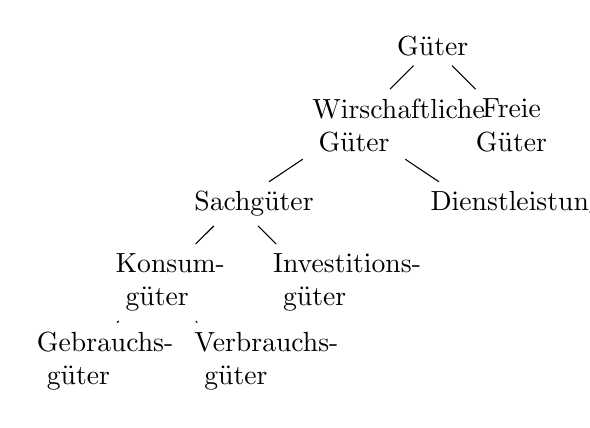
\begin{tikzpicture}[grow=down, sloped]
\node[box] {Güter}
		child {
		node[box] {Wirschaftliche Güter}
			child{
			node [box] {Sachgüter}
				child{
				node [box] {Konsum-güter}
					child{
					node [box] {Gebrauchs-güter}
					}
					child{
					node [box] {Verbrauchs-güter}
					}
				}
				child{
				node [box] {Investitions-güter}
				}
			}
			child{
			node [box] {Dienstleistungen}
			}
		}
		child {
		node [box] {Freie Güter}
		};
\end{tikzpicture}
\end{center}

Anmerkungen:
\begin{description}\itemsep0em
	\item [Freie Güter] sind gratis, weil unbeschränkt vorhandenen
	\item [Wirtschaftliche Güter] sind knapp (beschränkt vorhanden)
	\item [Dienstleistungen] sind nicht speicherbar (Verbrechen gelten als Dienstleistung)
	\item [Investitionsgüter] produzieren andere Güter (Private haben niemals Investitionsgüter) 
\end{description}

\subsection{Produktionsfaktoren}
\begin{description}\itemsep0em
	\item [Arbeit] Produktive Tätigkeit des Menschen
	\item [Natürliche Ressourcen] Boden und Rohstoffe
	\item [Realkapital] Maschinen, Anlagen, Gebäude
	\item [Wissen] Know how wie zu produzieren ist
\end{description}

\subsubsection{Prinzipien}
\begin{description}\itemsep0em
	\item [Maximierungsprinzip] Gegeben: Input, gesucht: maximales Ergebnis
	\item [Minimierungsprinzip] Gegeben: Ergebnis, gesucht: minimaler Input
\end{description}


\subsection{Arbeitsteilung, Tausch, Geld}
Arbeitsteilung und Spezialisierung entschärfen das Knappheitsproblem, weil sich dadurch
die Produktivität und infolgedessen das Gütervolumen erhöhen lässt.

Ohne Geld wäre direkter Tausch (Wand anstreichen gegen Kartoffeln) erforderlich.
Mit Hilfe von Geld geht es indirekt:
\begin{equation*}
	\mbox{wirtschaftliches Gut} \Leftrightarrow \mbox{Geld} \Leftrightarrow \mbox{wirtschaftliches Gut}
\end{equation*}

\begin{description}\itemsep0em
	\item [Transaktionskosten] sind die Summe aller Kosten, die erforderlich sind, um einen Handel abzuwickeln, die aber nicht mit dem Handel selbst zu tun haben
	\item [Opportunitätskosten] stehen für entgangenen Nutzen, der dadurch entsteht, dass vorhandene Möglichkeiten nicht genutzt werden. (Nichts ist gratis)
	\begin{equation*}
		\mbox{Maximaler Nutzen} \Leftrightarrow \mbox{Minimale Opportunitätskosten}
	\end{equation*}
	\item [Trade-off] Bezeichnet die Konkurrenz von Zielen. Das keine kann nur zu Lasten des anderen erreicht werden (Je mehr dies, desto weniger das).
\end{description}

Knappheit und Tausch spielen in der Volkswirtschaftslehre eine so grosse Rolle,
dass man das gesamte Gebiet oft als die Lehre von \enquote{Entscheidungen bei Knappheit}
oder als die Lehre vom Tausch bezeichnet.

